\documentclass[conference]{IEEEtran}

\usepackage{cite}
\usepackage{amsmath}
\usepackage{graphicx}
\usepackage{url}

\begin{document}

\title{A Federated Learning Approach for Layer 2 Network Intrusion Detection\\
with Explainable AI Across Distributed Network Segments}

\author{
\IEEEauthorblockN{Hosein Ghasemizade}
\IEEEauthorblockA{\textit{Department of Computer Engineering} \\
\textit{Central Tehran Branch}\\
Tehran, Iran\\
ghasemizade.hosein@gmail.com}
}

\maketitle

\begin{abstract}
The rapid expansion of networked environments, the proliferation of IoT devices, and
increasing reliance on cloud services have significantly broadened the attack surface of
modern networks. While existing Intrusion Detection Systems (IDS) primarily operate at
Layer~3 and above, critical attacks such as ARP Spoofing, MAC Flooding, DHCP Starvation,
and STP-based exploits occur at the Data Link Layer (Layer~2) and evade traditional
IP-based detection mechanisms. This paper proposes a federated learning framework for
Layer~2 network intrusion detection that integrates a hybrid CNN-BiLSTM deep learning
model with Explainable AI (XAI) techniques. By leveraging the FedProx aggregation
algorithm, the system addresses Non-IID data heterogeneity across distributed network
segments without transmitting raw traffic data, thereby preserving privacy. SHAP
(SHapley Additive exPlanations) is employed to interpret model decisions, enhancing
transparency and trust for security analysts. The proposed framework is evaluated against
centralized baselines across varied heterogeneity conditions, with performance measured in
terms of accuracy, F1-score, false alarm rate, communication overhead, and computational
resource consumption. The research targets practical deployment on resource-constrained
hardware and is applicable to enterprise networks, IoT infrastructures, and edge
computing environments.
\end{abstract}

\begin{IEEEkeywords}
Federated Learning, Intrusion Detection System, Layer~2 Security, Explainable AI,
SHAP, CNN-BiLSTM, FedProx, Non-IID, ARP Spoofing, MAC Flooding
\end{IEEEkeywords}

\section{Introduction}

Network security has become a critical concern due to the increasing dependence on interconnected systems, cloud infrastructures, and IoT environments. Intrusion Detection Systems (IDSs) are widely deployed to identify malicious activities and unauthorized access attempts within network infrastructures. However, most existing IDS solutions concentrate on network-layer and application-layer attacks while providing limited protection against attacks occurring at the Data Link Layer.

Layer 2 attacks such as ARP Spoofing, MAC Flooding, DHCP Starvation, and DHCP Spoofing can compromise local area networks before higher-layer security mechanisms become effective. Detecting these attacks remains challenging because they often leave minimal traces in IP-based traffic analysis.

Recent advances in deep learning have improved IDS performance, but centralized training approaches require collecting large amounts of raw network traffic, resulting in privacy and scalability limitations. Federated Learning (FL) offers an alternative by enabling collaborative model training without sharing raw data. Nevertheless, the application of FL to Layer 2 intrusion detection remains largely unexplored.

This paper proposes a privacy-preserving and explainable Layer 2 IDS framework that integrates Federated Learning, CNN-BiLSTM deep learning models, and SHAP-based Explainable AI.

\section{Related Work}

Recent studies have explored deep learning approaches for intrusion detection using architectures such as CNN, LSTM, and Bi-LSTM. These models have demonstrated high detection accuracy for various cyberattacks but primarily focus on Layer 3 and above.

Research on Layer 2 intrusion detection remains limited. Systems such as BCAST IDS and CL2-IDS have shown promising results in identifying MAC-level attacks through traffic behavior analysis. However, these approaches are generally centralized and do not address privacy-preserving distributed learning.

Federated Learning has gained attention in IDS research because of its ability to preserve data privacy and reduce communication overhead. Existing FL-based IDS solutions mainly target IoT and higher-layer network traffic. Similarly, Explainable AI techniques such as SHAP have been applied to enhance transparency in security-related machine learning systems. However, integrating FL, XAI, and Layer 2 IDS remains an open research problem.

\section{Proposed Framework}

The proposed architecture consists of multiple distributed network segments acting as federated clients and a central aggregation server.

Each client collects Layer 2 traffic data and performs local model training using a hybrid CNN-BiLSTM architecture. The CNN component extracts spatial traffic features, while the Bi-LSTM captures temporal dependencies within packet sequences.

Instead of transmitting raw traffic data, clients send model updates to a central server. The server aggregates local parameters using the FedProx algorithm, which is specifically designed to handle non-IID data distributions.

To improve transparency, SHAP is employed to explain model predictions and identify the most influential Layer 2 traffic features contributing to attack detection decisions.

Figure~\ref{fig:framework} illustrates the proposed framework.

\begin{figure}[htbp]
\centering
 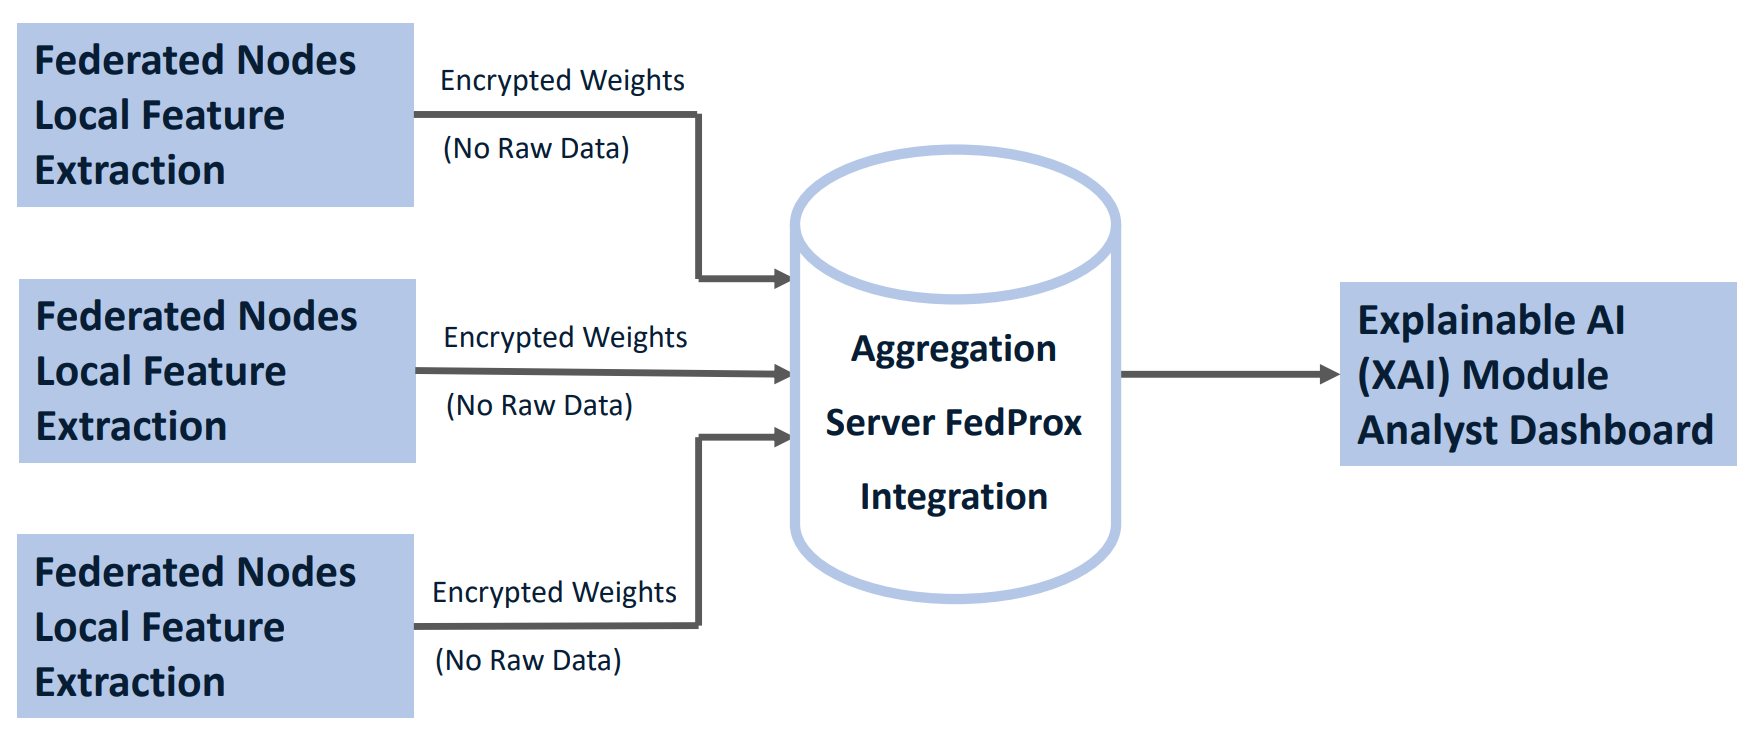
\includegraphics[width=0.45\textwidth]{framework.png}
\caption{Conceptual architecture of the proposed Federated Layer 2 IDS.}
\label{fig:framework}
\end{figure}

\section{Research Methodology}

The proposed study follows an experimental research methodology.

Initially, Layer 2 attack datasets including CL2-IDS and BCAST IDS will be collected and preprocessed. Traffic records will be normalized and distributed among federated clients under both IID and Non-IID settings.

The CNN-BiLSTM model will be trained locally on each client node. After each training round, model parameters will be transmitted to the aggregation server, where FedProx will generate a global model.

To evaluate robustness under heterogeneous environments, FedProx will be compared with FedAvg. Furthermore, SHAP analysis will be performed to investigate feature importance and improve model interpretability.

Performance evaluation will be conducted using:

\begin{itemize}
\item Accuracy
\item Precision
\item Recall
\item F1-Score
\item False Alarm Rate
\item AUC-ROC
\item Communication Overhead
\item CPU and Memory Consumption
\item Inference Latency
\end{itemize}

The feasibility of deployment on resource-constrained devices such as Raspberry Pi will also be assessed.

\section{Expected Results and Discussion}

The proposed framework is expected to achieve detection performance comparable to centralized IDS systems while preserving user privacy through federated learning.

The CNN-BiLSTM model is anticipated to improve the identification of Layer 2 attack patterns due to its ability to learn both spatial and temporal traffic characteristics. FedProx is expected to outperform FedAvg under Non-IID conditions by improving model convergence and stability.

Moreover, SHAP explanations should provide meaningful insights into model decisions, thereby enhancing analyst trust and facilitating forensic investigations. The lightweight design is also expected to enable deployment in edge and IoT environments.

\section{Conclusion and Future Work}

This paper presented a research framework for a federated and explainable Layer 2 Intrusion Detection System. The proposed approach combines CNN-BiLSTM deep learning, FedProx-based federated learning, and SHAP-based Explainable AI to address challenges related to privacy, scalability, and interpretability.

Future work will focus on implementing the framework, conducting extensive experiments under real-world network conditions, and evaluating additional privacy-preserving mechanisms such as Differential Privacy and Secure Aggregation.

\bibliographystyle{IEEEtran}

\begin{thebibliography}{99}

\bibitem{Belenguer2025}
A. Belenguer, J. A. Pascual, and J. Navaridas,
``A Review of Federated Learning Applications in Intrusion Detection Systems,''
\emph{Computer Networks}, 2025.

\bibitem{Chinnasamy2025}
R. Chinnasamy et al.,
``Deep Learning-Driven Methods for Network-Based Intrusion Detection Systems: A Systematic Review,''
\emph{ICT Express}, 2025.

\bibitem{Gombao2025}
J. Gombao,
``BCAST IDS: A Novel Network Intrusion Detection System,''
\emph{IEEE Access}, 2025.

\bibitem{Kilincer2025}
I. F. Kilincer,
``Explainable AI Supported Hybrid Deep Learning Method for Layer 2 Intrusion Detection,''
\emph{Egyptian Informatics Journal}, 2025.

\bibitem{Verkerken2023}
M. Verkerken et al.,
``A Novel Multi-Stage Approach for Hierarchical Intrusion Detection,''
\emph{IEEE Transactions on Network and Service Management},
vol. 20, no. 3, pp. 3915--3929, 2023.

\end{thebibliography}

\end{document}